\section{Trigonometría}
\begin{itemize}
	\item Ángulos notables
	\begin{table}[H]
		\centering
		\begin{tabular}{|c|c|c|c|c|c|c|c|}
			\hline
			& $0$ & $30^{\circ}$ & $45^{\circ}$ & $60^{\circ}$ & $90^{\circ}$ & $180^{\circ}$ & $270^{\circ}$ \\
			\hline
			$\msin{x}$ & $0$ & $\dfrac{1}{2}$ & $\dfrac{\sqrt{2}}{2}$ & $\dfrac{\sqrt{3}}{2}$ & $1$ & $0$ & $-1$ \\
			\hline
			$\mcos{x}$ & $1$ & $\dfrac{\sqrt{3}}{2}$ & $\dfrac{\sqrt{2}}{2}$ & $\dfrac{1}{2}$ & $0$ & $-1$ & $0$ \\
			\hline
			$\mtan{x}$ & $0$ & $\dfrac{\sqrt{3}}{3}$ & $1$ & $\sqrt{3}$ & -- & $0$ & -- \\
			\hline
			$\mcot{x}$ & -- & $\sqrt{3}$ & $1$ & $\dfrac{\sqrt{3}}{3}$ & $0$ & -- & $0$ \\
			\hline
			$\msec{x}$ & $1$ & $\dfrac{2\sqrt{3}}{3}$ & $\sqrt{2}$ & $2$ & -- & $-1$ & -- \\
			\hline
			$\mcsc{x}$ & -- & $2$ & $\sqrt{2}$ & $\dfrac{2\sqrt{3}}{3}$ & $1$ & -- & $1$ \\
			\hline
		\end{tabular}
	\end{table}
	\item Leyes de senos, cosenos, tangentes y proyecciones
	\begin{figure}[H]
		\centering
		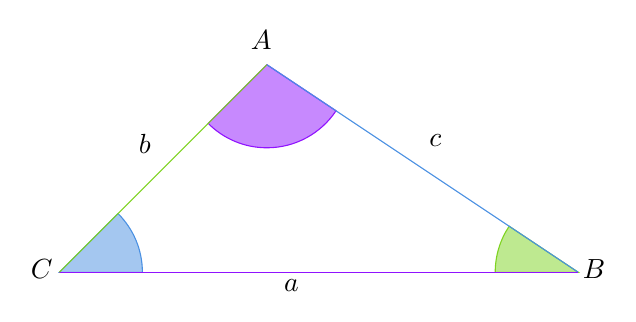
\begin{tikzpicture}[x=0.75pt,y=0.75pt,yscale=-1,xscale=1]
			%uncomment if require: \path (0,300); %set diagram left start at 0, and has height of 300
			
			%Shape: Pie [id:dp43438130853596024] 
			\draw  [color={rgb, 255:red, 144; green, 19; blue, 254 }  ,draw opacity=1 ][fill={rgb, 255:red, 144; green, 19; blue, 254 }  ,fill opacity=0.5 ] (153.29,42.19) .. controls (146.11,52.93) and (133.88,60) .. (120,60) .. controls (108.95,60) and (98.95,55.52) .. (91.72,48.28) -- (120,20) -- cycle ;
			%Shape: Pie [id:dp8399272714698878] 
			\draw  [color={rgb, 255:red, 126; green, 211; blue, 33 }  ,draw opacity=1 ][fill={rgb, 255:red, 126; green, 211; blue, 33 }  ,fill opacity=0.5 ] (230,120) .. controls (230,120) and (230,120) .. (230,120) .. controls (230,111.79) and (232.47,104.16) .. (236.71,97.81) -- (270,120) -- cycle ;
			%Shape: Pie [id:dp5872530047217905] 
			\draw  [color={rgb, 255:red, 74; green, 144; blue, 226 }  ,draw opacity=1 ][fill={rgb, 255:red, 74; green, 144; blue, 226 }  ,fill opacity=0.5 ] (48.28,91.72) .. controls (55.52,98.95) and (60,108.95) .. (60,120) -- (20,120) -- cycle ;
			%Straight Lines [id:da2492814789045239] 
			\draw [color={rgb, 255:red, 74; green, 144; blue, 226 }  ,draw opacity=1 ]   (120,20) -- (270,120) ;
			%Straight Lines [id:da9401030907167269] 
			\draw [color={rgb, 255:red, 144; green, 19; blue, 254 }  ,draw opacity=1 ]   (20,120) -- (270,120) ;
			%Straight Lines [id:da1561250698698038] 
			\draw [color={rgb, 255:red, 126; green, 211; blue, 33 }  ,draw opacity=1 ]   (120,20) -- (20,120) ;
			
			% Text Node
			\draw (111,2.4) node [anchor=north west][inner sep=0.75pt]    {$A$};
			% Text Node
			\draw (271,112.4) node [anchor=north west][inner sep=0.75pt]    {$B$};
			% Text Node
			\draw (5,112.4) node [anchor=north west][inner sep=0.75pt]    {$C$};
			% Text Node
			\draw (127,122.4) node [anchor=north west][inner sep=0.75pt]    {$a$};
			% Text Node
			\draw (57,52.4) node [anchor=north west][inner sep=0.75pt]    {$b$};
			% Text Node
			\draw (197,52.4) node [anchor=north west][inner sep=0.75pt]    {$c$};
			
			
		\end{tikzpicture}
	\end{figure}
	\begin{itemize}
		\item Ley de senos
		\[ \dfrac{a}{\msin{A}} =\dfrac{b}{\msin{B}} =\dfrac{c}{\msin{C}} \]
		\item Ley de cosenos
		\begin{align*}
			a^{2} &= b^{2} + c^{2} - 2bc\mcos{A} \\
			b^{2} &= a^{2} + c^{2} - 2ac\mcos{B} \\
			c^{2} &= a^{2} + b^{2} - 2ab\mcos{C} 
		\end{align*}
		\item Ley de tangentes
		\begin{align*}
			\dfrac{a + b}{a - b} &=\dfrac{\mtan{\frac{A + B}{2}}}{\mtan{\frac{A - B}{2}}} \\
			\dfrac{a + c}{a - c} &=\dfrac{\mtan{\frac{A + C}{2}}}{\mtan{\frac{A - C}{2}}} \\
			\dfrac{b + c}{b - c} &=\dfrac{\mtan{\frac{B + C}{2}}}{\mtan{\frac{B - C}{2}}}
		\end{align*}
		\item Ley de proyecciones
		\begin{align*}
			a\mcos{B} + b\mcos{A} &= c \\
			a\mcos{C} + c\mcos{A} &= b \\
			b\mcos{C} + c\mcos{B} &= a
		\end{align*}
	\end{itemize}
	\item $\ds\msin{-x} =-\msin{x}$
	\item $\ds\mcos{-x} =\mcos{x}$
	\item $\ds\msin{x}\mcsc{x} = 1$
	\item $\ds\mcos{x}\msec{x} = 1$
	\item $\ds\mtan{x}\mcot{x} = 1$
	\item $\ds\mtan{x} =\dfrac{\msin{x}}{\mcos{x}} =\dfrac{1}{\mcot{x}}$
	\item $\ds\mcot{x} =\dfrac{\mcsc{x}}{\msec{x}} =\dfrac{1}{\mtan{x}}$
	\item $\ds\msin{x}[2] +\mcos{x}[2] = 1$
	\item $\ds\mtan{x}[2] + 1 =\msec{x}[2]$
	\item $\ds\mcot{x}[2] + 1 =\mcsc{x}[2]$
	\item $\ds\msin{x\pm y} =\msin{x}\mcos{y}\pm\mcos{x}\msin{y}$
	\item $\ds\mcos{x\pm y} =\mcos{x}\mcos{y}\mp\msin{x}\msin{y}$
	\item $\ds\mtan{x\pm y} =\dfrac{\mtan{x}\pm\mtan{y}}{1\mp\mtan{x}\mtan{y}}$
	\item $\ds\msin{2x} =2\msin{x}\mcos{x}$
	\item $\ds\mcos{2x} =\mcos{x}[2] -\msin{x}[2]$
	\item $\ds\mcos{2x} = 1 - 2\msin{x}[2] = 2\mcos{x}[2] - 1$
	\item $\ds\mtan{2x} =\dfrac{2\mtan{x}}{1 -\mtan{x}[2]}$
	\item $\ds\msin{\dfrac{x}{2}} =\pm\sqrt{\dfrac{1 -\mcos{x}}{2}}$
	\item $\ds\mcos{\dfrac{x}{2}} =\pm\sqrt{\dfrac{1 +\mcos{x}}{2}}$
	\item $\ds\mtan{\dfrac{x}{2}} =\pm\sqrt{\dfrac{1 - \mcos{x}}{1 +\mcos{x}}}$
	\item $\ds\mtan{\dfrac{x}{2}} =\dfrac{1 -\mcos{x}}{\msin{x}} =\dfrac{\msin{x}}{1 +\mcos{x}}$
	\item $\ds\msin{x}\pm\msin{y} =2\msin{\dfrac{x\pm y}{2}}\mcos{\dfrac{x\mp y}{2}}$
	\item $\ds\mcos{x + y} = 2\mcos{\dfrac{x + y}{2}}\mcos{\dfrac{x - y}{2}}$
	\item $\ds\mcos{x - y} = -2\msin{\dfrac{x + y}{2}}\msin{\dfrac{x - y}{2}}$
	\item $\ds\msin{x}\msin{y} =\dfrac{1}{2}\pa{\mcos{x - y} -\mcos{x + y}}$
	\item $\ds\mcos{x}\mcos{y} =\dfrac{1}{2}\pa{\mcos{x - y} +\mcos{x + y}}$
	\item $\ds\msin{x}\mcos{y} =\dfrac{1}{2}\pa{\msin{x + y} +\msin{x - y}}$
\end{itemize}